%%%%% Please set the path to 'beamer' directory in your environment %%%%%
\newcommand{\beamerDir}[0]{/mnt/c/Users/atsushi/Documents/workspace/env/Beamer/beamer/beamer/}


%%%%% Load setting %%%%%
\documentclass[aspectratio=169, dvipdfmx, 12pt, compress]{beamer}% dvipdfmxしたい

%%%%% Packages %%%%%
\usepackage{bxdpx-beamer}% dvipdfmxなので必要
\usepackage{pxjahyper}% 日本語で'しおり'したい
\usepackage{tikz}
\usepackage{tcolorbox}
\usetikzlibrary{shapes}
\usepackage{xcolor}
\usepackage[absolute,overlay]{textpos}
\usepackage{adjustbox}
\usepackage{caption}
\usepackage{ifthen}


%%%%% Settings %%%%%
\usetheme[sectionpage=progressbar, subsectionpage=progressbar]{metropolis}
% block style
\metroset{block=fill}
% space between line
\renewcommand{\baselinestretch}{1.3}
% space between item
\newlength{\wideitemsep}
\setlength{\wideitemsep}{0.9\itemsep}
% \addtolength{\wideitemsep}{1.0pt} <- more space
\let\olditem\item
\renewcommand{\item}{\setlength{\itemsep}{\wideitemsep}\olditem}
% frame title
\definecolor{coolblack}{rgb}{0.0, 0.18, 0.39}
\setbeamercolor{frametitle}{bg=coolblack!90,fg=white}
\setbeamerfont{frametitle}{size=\large}
\addtobeamertemplate{frametitle}{}{\vspace{-1em}}
\makeatletter
\setlength{\metropolis@frametitle@padding}{1.4ex}% <- default 2.2 ex
% foot line
\addtobeamertemplate{footline}{}{\vspace{-1em}}
% normal text color
\setbeamercolor{normal text}{fg=black!80}
% progress bar
\definecolor{lightgray}{rgb}{0.83, 0.83, 0.83}
\setbeamercolor{progress bar}{bg=lightgray, fg=coolblack}
\setbeamersize{text margin left=15pt, text margin right=15pt}
% equation font
\usefonttheme{professionalfonts}
% Change standard block width
\addtobeamertemplate{block begin}{%
    \centering
    \begin{columns}\begin{column}{0.9\textwidth}
            \centering
            }{}
            \addtobeamertemplate{block end}{}{\end{column}\end{columns}}
% Change alert block width
\addtobeamertemplate{block alerted begin}{%
    \centering
    \begin{columns}\begin{column}{0.9\textwidth}
            \centering
            }{}
            \addtobeamertemplate{block alerted end}{}{\end{column}\end{columns}}
% Change example block width
\addtobeamertemplate{block example begin}{%
    \centering
    \begin{columns}\begin{column}{0.9\textwidth}
            \centering
            }{}
            \addtobeamertemplate{block example end}{}{\end{column}\end{columns}}
% Itemize color
\setbeamertemplate{itemize item}{\color{black}\scriptsize$\blacksquare$}
\setbeamertemplate{itemize subitem}{\color{black}\scriptsize$-$}
% Simplification  color
\definecolor{cobalt}{rgb}{0.0, 0.28, 0.67}
\setbeamercolor{block title example}{fg=black!80,bg=cobalt!35}
\setbeamercolor{block body example}{fg=black,bg=cobalt!15}
% Definition
\BeforeBeginEnvironment{definition}{
    \setbeamercolor{block title}{use=alerted text, bg=alerted text.fg!70,fg=white}
    \setbeamercolor{block body}{use=alerted text, bg=alerted text.fg!20}
}
\AfterEndEnvironment{definition}{% return to default
    \setbeamercolor{block title}{use=structure,fg=structure.fg,bg=structure.fg!20!bg}
    \setbeamercolor{block body}{parent=normal text,use=block title,bg=block title.bg!50!bg, fg=black}
}
% Theorem
\definecolor{seagreen}{rgb}{0.18, 0.55, 0.34}
\setbeamertemplate{theorems}[numbered]
\BeforeBeginEnvironment{theorem}{
    \setbeamercolor{block title}{fg=black!80,bg=seagreen!40}
    \setbeamercolor{block body}{fg=black,bg=seagreen!15}
}
\AfterEndEnvironment{theorem}{% return to default
    \setbeamercolor{block title}{use=structure,fg=structure.fg,bg=structure.fg!20!bg}
    \setbeamercolor{block body}{parent=normal text,use=block title,bg=block title.bg!50!bg, fg=black}
}
% Lemma
\undef{\lemma}
\newtheorem{lemma}{\translate{Lemma}}
\BeforeBeginEnvironment{lemma}{
    \setbeamercolor{block title}{fg=black!80,bg=seagreen!20}
    \setbeamercolor{block body}{fg=black,bg=seagreen!10}
}
\AfterEndEnvironment{lemma}{% return to default
    \setbeamercolor{block title}{use=structure,fg=structure.fg!80,bg=structure.fg!20!bg}
    \setbeamercolor{block body}{parent=normal text,use=block title,bg=block title.bg!50!bg, fg=black}
}


%%%%% Original Command %%%%%
\newcommand{\subt}[1]{\vspace{-2mm}{\fontsize{10pt}{0cm}\selectfont \textcolor{lightgray}{#1}}\vspace{-1mm}}
\newcommand{\lastpage}[0]{\begin{frame}\begin{textblock*}{1.0\linewidth}(0pt, 50pt)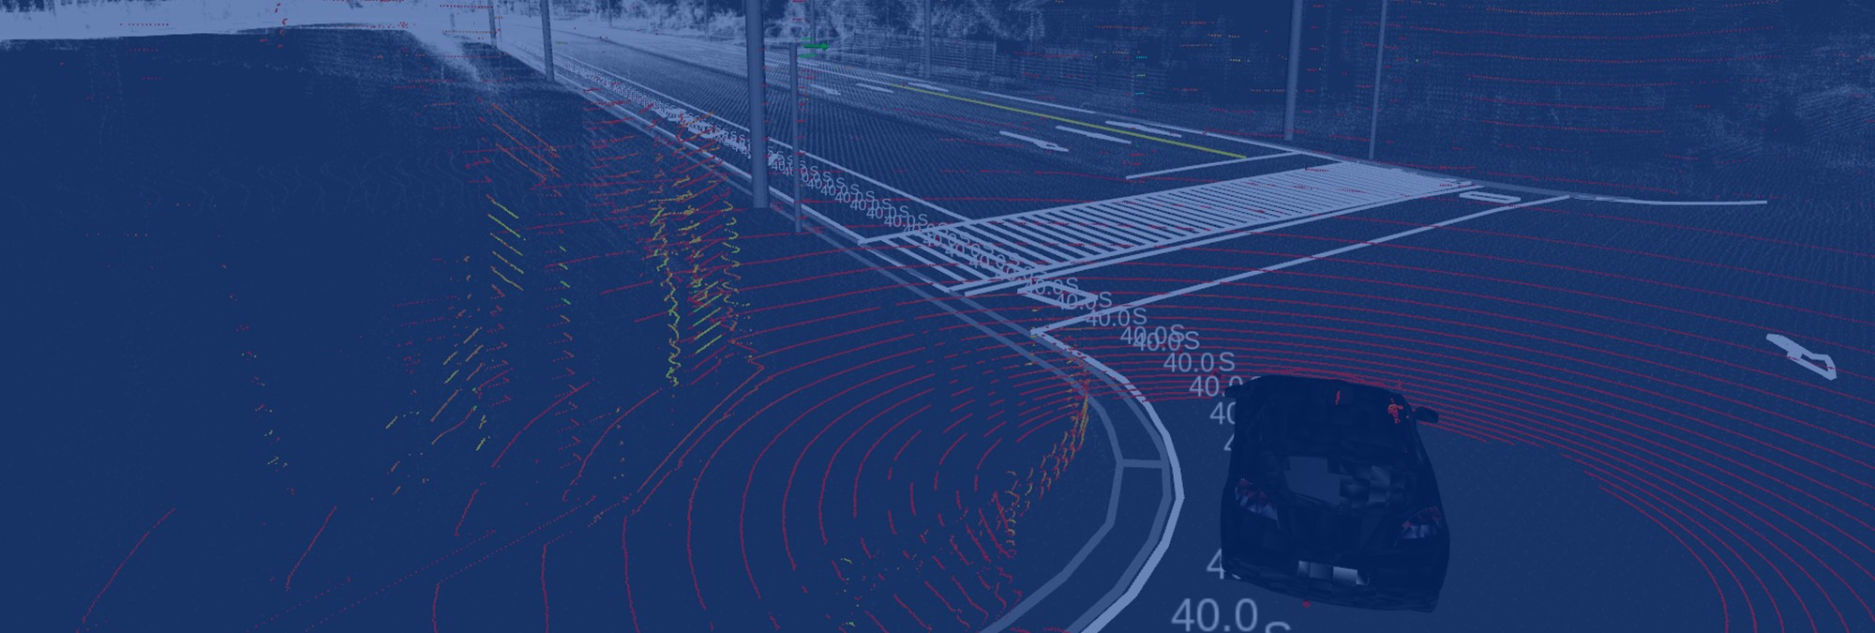
\includegraphics[scale=0.512]{\beamerDir/master_figure/last.pdf}\end{textblock*}\end{frame}}
\newcommand{\todo}[1]{\al{\LARGE\textbf{TODO:} #1}}
\newcommand{\headerheight}[0]{5mm}
\newcommand{\footerheight}[0]{5mm}
\newcommand{\slideheight}[0]{\textheight-\headerheight-\footerheight}
\newcommand{\tabml}[1]{\hspace{-2.1mm}\begin{tabular}{l} #1 \end{tabular}}
\newcommand{\al}[1]{\alert{#1}}
\newcommand{\argempty}[0]{}
\newcommand{\onlyslide}[1]{
    \vspace{\headerheight}
    \begin{minipage}[c][\slideheight][c]{\textwidth}
        #1
    \end{minipage}
}
\newcommand{\onlyimage}[1]{
    \onlyslide{
        \centering
        \begin{columns}
            \begin{column}{\textwidth}
                \centering
                \adjustbox{max width=\textwidth, max height=\slideheight}{
                    \includegraphics{#1}
                }
            \end{column}
        \end{columns}
    }
}
% fit image
\newlength\fitimageht
\newlength\fitotherht
\newsavebox\fitimagebox
\newcommand{\fitimage}[2]{%
    \sbox\fitimagebox{%
        \parbox{\textwidth}{%
            #1\par
        }%
    }%
    \settototalheight{\fitotherht}{%
        \usebox\fitimagebox
    }%
    \setlength\fitimageht{\textheight}%
    \addtolength\fitimageht{-\fitotherht-\headerheight-\footerheight-1\baselineskip}%
    \vspace{\headerheight}
    #1\par
    \centering
    \includegraphics[width=\textwidth,height=\fitimageht,keepaspectratio]{#2}
}
% Simplification
\newcommand{\assume}[1]{
    \begin{exampleblock}{Simplification }
        #1
    \end{exampleblock}
}
% Re-post
\setbeamercolor{RepostBox}{fg=black!50, bg=coolblack!10}
\newcommand{\repost}[1]{
    \vspace{2mm}
    \centering
    \begin{columns}
        \begin{column}{0.86\textwidth}
            \begin{beamercolorbox}[wd=\textwidth, sep=2pt, rounded=true, shadow=true]{RepostBox}
                \begin{tabular}{|p{0.95\textwidth}}
                    {\fontsize{10pt}{10pt}#1}
                \end{tabular}
            \end{beamercolorbox}
        \end{column}
    \end{columns}
}

% equation ballon
\tcbset{
    framebox/.style={
            enhanced,
            boxsep=0pt,       % 箱の上下左右の余白を指定
            colback=white,
            boxrule=1pt,
            colframe=#1
        },
    framebox/.default=red
}
\newcommand{\upbln}[3]{
    \tcboxmath[
        framebox=#2,
        top=0.5ex,bottom=0.5ex,    % 箱の上下の余白を指定
        left=0.5ex,right=0.5ex,    % 箱の左右の余白を指定
        overlay={
                \node[
                    above,
                    rectangle callout,                         % nodeを吹き出しの形に
                    callout absolute pointer={(frame.north)},  % 吹き出しの先端を絶対的に指定
                    fill=#2!20
                ] at ([yshift=2ex]frame.north) {\footnotesize#3};
            }
    ]{#1}
}
\newcommand{\lwbln}[3]{
    \tcboxmath[
        framebox=#2,
        top=0.5ex,bottom=0.5ex,    % 箱の上下の余白を指定
        left=0.5ex,right=0.5ex,    % 箱の左右の余白を指定
        overlay={
                \node[
                    below,
                    rectangle callout,                         % nodeを吹き出しの形に
                    callout absolute pointer={(frame.south)},  % 吹き出しの先端を絶対的に指定
                    fill=#2!20
                ] at ([yshift=-2ex]frame.south) {\footnotesize#3};
            }
    ]{#1}
}
\tcbuselibrary{theorems,skins}



%%%%% Mode %%%%%
% \newcommand{\forme}[1]{#1}
\newcommand{\forme}[1]{}


%%%%% Front Cover %%%%%
\title{HMDS: A Makespan Minimizing DAG Scheduler for Heterogeneous Distributed Systems}
\subtitle{ACM Transactions on Embedded Computing Systems (TECS), 2021}
\author{矢野 篤志}
% \date{\today}
\institute[EMBIV]{EMBIV}
\logo{\begin{textblock*}{0.1\linewidth}(2pt, 237pt)
\includegraphics[scale=0.4]{\beamerDir/master_figure/Emb_logo.pdf}\end{textblock*}}


%%%%% Document Start %%%%%
\begin{document}

\maketitle

\summary{2}{0}
% !TeX root = main.tex


\begin{frame}{提案の概要}
    \begin{itemize}
        \item 優先度駆動型スケジューリングによってROSのリアルタイム性能と予測可能性を大幅に改善できることを主張する
        \item 主張を裏付けるために, 優先度駆動型チェーン考慮スケジューリングに関する我々の研究をレビューし, Apex.AI が開発したオープンソースリファレンスシステムを用いた評価を行う
        \item ROS 2のリアルタイム性能を向上させるために不可欠な以下2つの課題を説明する
        \begin{itemize}
            \item マルチスレッドエグゼキュータ設計
            \item アクセラレータサポート
        \end{itemize}
    \end{itemize}
\end{frame}


\begin{frame}{Outline}
    \setbeamertemplate{section in toc}[sections numbered]
    \scriptsize\tableofcontents[hideallsubsections]
\end{frame}

% % !TeX root = main.tex

\section{PRIOR KNOWLEDGE}
\label{sec: prior knowledge}

\begin{frame}{前提知識}
    \begin{itemize}
        \item \ourl{ROS}{https://tier4.atlassian.net/wiki/spaces/EMBIV/pages/2683603071/ROS+Robot+Operating+System}
        \item \ourl{publish/subscribeモデル}{https://tier4.atlassian.net/wiki/spaces/EMBIV/pages/2675048610/Publish+Subscribe}
        \item \ourl{SCHED\_DEADLINE}{https://tier4.atlassian.net/wiki/spaces/EMBIV/pages/2692645566/SCHED+DEADLINE}
        \item \ourl{最大イベント到着曲線}{https://drive.google.com/file/d/1n85X0vDrDm4IDANDP4aUoC0SNnZLAiRN/view?usp=share_link}
        \item \ourl{Casiniらによる先行研究}{https://drive.google.com/file/d/1sHujFqbmgCoJbC6g6KdC7ihua4Jqddju/view?usp=share_link}
    \end{itemize}
\end{frame}

% % !TeX root = main.tex

\section{INTRODUCTION}
\label{sec: introduction}

\begin{frame}{}
    \begin{itemize}
        \item ロボット工学のような, 様々な分野の深い専門知識を必要とする学際的で複雑なアプリケーション領域では, 通常, 全ての, あるいはほとんどのソフトウェアをゼロから書くという選択肢はあり得ない
        \item その代わりに, ロボット工学者は, ROSのような一般的なロボット工学フレームワークで容易に利用できる, 標準機能を提供する既存のサードパーティコンポーネントの統合を採用するのが一般的である
        \item その利点は数多く, 簡単に理解できる
        \item 例えば, 複数の最新パス計画アルゴリズムと3D可視化サポートを備えた完全なナビゲーションスタックがたった1回のダウンロードで手に入るなら, なぜ新しいナビゲーションサブシステムを苦労して開発する必要があるか?
    \end{itemize}
\end{frame}

\begin{frame}{}
    \begin{itemize}
        \item 完全なロボットシステムを構築するためには, 多くの相互作用するコンポーネントを統合する必要がある
        \item ROS開発プロセスの分散型オープンソースの性質により, これらのコンポーネントは通常, 必ずしもお互いを知らない複数の独立したコンポーネント開発者によって分離して開発される
        \item 同様に, システムインテグレータは, アプリケーションおよびミッション固有のロジックと「グルーコード」で展開プラットフォーム上で選択したコンポーネントを構成するが, 通常, それぞれのコンポーネント開発者と密接に連携することはない
    \end{itemize}
\end{frame}

\begin{frame}{}
    \begin{itemize}
        \item コンポーネントの統合を可能な限りシンプルに保つために, ROSはコンポーネントの疎結合を可能にする古典的なトピックベースのpublish/subscribeパラダイムを採用している
        \item 概念的には, 各コンポーネントは, 特定のトピックをsubscribeする多数のコールバックを含む「ブラックボックス」として理解できる
        \item 与えられたトピックに関連するメッセージがpublishされるたびに, 全てのsubscribeコールバックが呼び出され, 何らかの計算を実行し, 次に他のトピックに後続のメッセージをpublishすることができ, これがさらにコールバックをトリガするというように, 繰り返す
    \end{itemize}
\end{frame}

\begin{frame}{}
    \begin{itemize}
        \item インテグレータは, あるコンポーネントの「入力コールバック」を別のコンポーネントの「出力トピック」に接続することによってコンポーネントを構成する
        \item ROSシステムは, このように相互接続されたトピックとコールバックの複雑なネットワークを形成し, データ (環境刺激など) は, イベント駆動型の方法でネットワークを通じてcause-effectチェーンに沿って伝播し, インテグレータが望むように透過的にコンポーネント境界を交差させることができる
    \end{itemize}
\end{frame}

\begin{frame}{}
    \begin{itemize}
        \item このようなcause-effectチェーンの典型的な例として, 進路上の障害物を検知して反応する必要のある移動ロボットのセンシング-計算-行動パイプラインが挙げられる
        \item 例えば, ハードウェアドライバコンポーネントがレーザースキャナから新しいサンプルを取得し (cause) , それが複数のマッピング, 座標変換, パス計画, 車輪制御コンポーネントを経て, 最終的に車輪速度の変化 (effect) をもたらす可能性がある
        \item このようなデータ処理のチェーンにおいて, causeからeffectまでの最大レイテンシ時間は, ロボットが正しく機能するために重要な役割を果たすことは明らかであり, また, 安全性を考慮する上でも重要であることが多い
    \end{itemize}
\end{frame}

\begin{frame}{}
    \begin{itemize}
        \item 重要なのは, システムインテグレータにできるだけ多くの展開の選択肢を残し, コンポーネントの再利用の機会を最大化するために, ROSの実行管理層と基礎となるオペレーティングシステムは, 意図的にコンポーネント開発者に公開されないことである
        \item むしろ, ROSの中心的なコールバック抽象化は, コールバック手続きがいつどのようにスケジュールされるか, コールバックの実行がスレッドまたはプロセスにわたってどのように組織されるか, またはネットワーキング層がメッセージの送受信をどのように処理するかを全く意識せずに, 実行から完了までセマンティクスを持つ単なる手続きである
    \end{itemize}
\end{frame}

\begin{frame}{}
    \begin{itemize}
        \item ROSはオープンソースソフトウェアであるため, 原理的にはシステムの実行と通信の挙動を完全に理解し制御することが可能である
        \item このため, リアルタイムシステムの専門家から見れば, ROSにリアルタイムシステム研究でよく知られた技術を導入することは論理的なステップであるように思える可能性がある
        \item しかし, 一見したところ, これを難しくしているハードルがいくつかある
    \end{itemize}
\end{frame}

\begin{frame}{}
    \begin{itemize}
        \item まず第一に, インテグレータに必要な情報が不足している
        \item ほとんどのリアルタイム分析では, 同時実行タスクの数, それらの起動セマンティクスや機能的相互作用, メッセージの到着パターン, 最悪実行時間など, 多くの低レベルシステムの詳細に関する深い知識が前提となっている
        \item ROSコンポーネントは, この種の情報を提供するマニフェストと一緒に来ることはない
        \item さらに悪いことに, リアルタイム分析は, 欠陥のある情報や不完全な情報にうまく対処できない
        \item モデリング目的でサードパーティコンポーネントを手作業でリバースエンジニアリングしているときに, たった一つのミスや見落としがあれば, その取り組み全体を無条件に無効にしてしまうことになりかねない
    \end{itemize}
\end{frame}

\begin{frame}{}
    \begin{itemize}
        \item 第二に, 必要なシステムの詳細をコンポーネントレベルで静的に決定し, 記述することができない
        \item その理由のひとつは, 多くのロボット工学アルゴリズムが, ユースケースやプラットフォーム固有の側面に依存し, 実行時間や起動パターンが大きく変化するためである
        \item 例えば, ビデオストリーム中の物体を識別し, その軌跡を推測する一般的な物体追跡コンポーネントを考えてみよう (例えば, 隣の車線の車など)
        \item この機能の実行時間は, ビデオストリームのフレームレート, 解像度, コーデック, および特定のトラッキングアルゴリズムに関連する他の様々なパラメータを含む, 様々なパラメータに依存する
        \item これらのパラメータは, 一般的なオブジェクトトラッキングコンポーネントの開発者が前もって知っていたり, 固定されていたりするものではない
    \end{itemize}
\end{frame}

\begin{frame}{}
    \begin{itemize}
        \item このようなユースケース特有の情報は, 特定のロボットを構築するインテグレーターにしか分からない
        \item インテグレーターは, 必ずしもオブジェクトトラッキングやリアルタイムシステムの専門家ではないため, 特定の構成を選択した場合の影響を常に予測できるわけではない
        \item したがって, コンポーネントのリソース要求とリアルタイム動作は, 常に特定の展開で使用するという文脈で評価されなければならない
        \item これは, ROSフレームワークの人気の根底にある「ブラックボックス」コンポーネントのモジュール式再利用と相容れるものではない
    \end{itemize}
\end{frame}

\begin{frame}{}
    \begin{itemize}
        \item 最後に, 仮にインテグレータが各コンポーネントについてそれぞれの専門家と議論し, タイミング分析に必要な全ての詳細を入手できたとしても, 第三の根本的な問題が残る
        \item 多くのコンポーネントのリソース要件と性能特性は, 本質的にロボットの動的環境に依存し, したがって時間とともに変化するため, 静的 (最悪のケース) リソース配置は実行不可能なのである
    \end{itemize}
\end{frame}

\begin{frame}{}
    \begin{itemize}
        \item 例えば, 前述の物体追跡コンポーネントと, ランドマークベースの自己位置特定コンポーネントに依存するロボットを再度考えてみよう
        \item 一方, 人口が少ない田舎町よりも, にぎやかな街中を移動する方が, 物体追跡装置の処理時間はずっと長くなる
        \item 一方, 認識可能なランドマークが多い都市部では, ほぼ一様な風景よりも自己位置推定がはるかに容易である可能性が高い
        \item どちらの状況でも十分なリソースを確保するためには, システムインテグレーターは, 不毛の土地からなる賑やかな都市を想定したシステムを用意しなければならない
    \end{itemize}
\end{frame}

\begin{frame}{}
    \begin{itemize}
        \item ロボット工学では, このような悲観的なシステム設計を行うと, すぐに現実的な限界に直面することになる
        \item その代わりに, 実用的で費用対効果の高いシステムを維持するためには, 各コンポーネントのピーク需要の合計ではなく, 予想されるジョイントリソースのピーク需要に対してプロビジョニングを行う必要がある
    \end{itemize}
\end{frame}

\begin{frame}{貢献する}
    \begin{itemize}
        \item これらの課題を克服するために, 我々は, 実行時に動的にタイミングを考慮した方法でROSシステムをプロビジョニングするための自動レイテンシマネージャを使用することを提案する
        \item 具体的には, ROS Live latency manager (ROSLlama) を紹介する
        \item これは, 重要なcause-effectチェーンに沿ったレイテンシを, 非リアルタイム専門家が使いやすく, かつ設定にあまり手間をかけない方法で, 既存のリアルタイム機構を使用して制御することを可能にする
    \end{itemize}
\end{frame}

\begin{frame}{貢献する}
    \begin{itemize}
        \item ROS-Llamaは, 複雑なシステムパラメータをユーザに要求するのではなく, 実行時に必要なパラメータを自動的に推定し, 状況の変化に応じてスケジューリングパラメータを動的に調整することが可能である
        \item もし, 指定されたレイテンシの目標が全て同時に達成できない場合 (例えば, 不利な環境条件による一時的な過負荷が原因) , ROS-Llamaは制御された緩やかなデグレードプロセスを開始し, システムインテグレーターが純粋に宣言的な方法で (すなわち, cause-effectチェーンがどの部品を通過しているかを理解しなくても) cause-effectチェーンの重要性を特定できるようにする
    \end{itemize}
\end{frame}

\begin{frame}{本論文の貢献}
    \begin{itemize}
        \item  ロボティクス領域における動的レイテンシ管理問題を探求し, 実用的なソリューションが満たさなければならない制約と要件を文書化する (第III章)

        \item  ROSのための最初の自動レイテンシマネージャであるROS-Llamaの設計と実装を紹介する (セクションIV)

        \item 標準的な Linux システム上の ROS コンポーネントを用いて, ROS-Llama が移動ロボットのcause-effectチェーンのレイテンシをうまく制御できることを示す評価について報告する (セクションVI)

    \end{itemize}
\end{frame}

\begin{frame}{}
    \begin{itemize}
        \item ROS-Llamaは, 数年にわたる研究とエンジニアリングの努力の結果であり, その間, 我々は多くの課題や技術的な限界に遭遇した
        \item セクションVIIでは, 以下の点を強調する
              \begin{itemize}
                  \item  ROS-Llamaをより効果的かつ正確にするための分析改善の機会
                  \item  ROSとLinuxのプラットフォームには, システムのさらなる改良の妨げとなる大きな限界がある
              \end{itemize}
    \end{itemize}
\end{frame}

% % !TeX root = main.tex

\section{SYSTEM MODEL AND PROBLEM STATEMENT}
\label{sec: system model and problem statement}

\begin{frame}{}
    \begin{itemize}
        \item 始めに, 本論文で登場する表記法・用語の表を示す
        \item 基本的な表記法・用語は資料中で説明無しで使用する
        \item 別ファイルで開く・印刷するなどして, 常に参照できる状態にしておくことを推奨する
    \end{itemize}
\end{frame}

% !TeX root = main.tex

\begin{frame}{表記法・用語 1}
    \full{
        \begin{table}[tb]
            \adjustbox{max width=\textwidth, max height=\slideheight}{
                \centering\begin{tabular}{|c|l|} \hline
                    $m$                                                                                             & スレッド数                                                                                        \\\hline
                    $\Gamma=\left\{\mathcal{C}_{1}, \mathcal{C}_{2}, \cdots, \mathcal{C}_{|\Gamma|}\right\}$        & チェインのセット                                                                                  \\\hline
                    $|\Gamma|$                                                                                      & $\Gamma$内のチェインの数                                                                          \\\hline
                    $\mathcal{C}_{i}=\left\{c_{i, 1}, c_{i, 2}, \cdots, c_{i,\left|\mathcal{C}_{i}\right|}\right\}$ & チェイン                                                                                          \\\hline
                    $c_{i,j}$                                                                                       & $\mathcal{C}_{i}$の$j$番目のコールバック                                                          \\\hline
                    $\left|\mathcal{C}_{i}\right|$                                                                  & $\mathcal{C}_{i}$内のコールバックの数                                                             \\\hline
                    先行要素                                                                                        & $J_{i}^{k}$ 内の連続する要素 $c_{i, j}^{k}$ と $c_{i, j+1}^{k}$ の各ペアにおける $c_{i, j}^{k}$   \\\hline
                    後続要素                                                                                        & $J_{i}^{k}$ 内の連続する要素 $c_{i, j}^{k}$ と $c_{i, j+1}^{k}$ の各ペアにおける $c_{i, j+1}^{k}$ \\\hline
                    ソースコールバック                                                                              & $\mathcal{C}_{i}$ の最初のコールバック                                                            \\\hline
                    シンクコールバック                                                                              & $\mathcal{C}_{i}$ の最後のコールバック                                                            \\\hline
                \end{tabular}
            }
        \end{table}
    }
\end{frame}

\begin{frame}{表記法・用語 2}
    \full{
        \begin{table}[tb]
            \adjustbox{max width=\textwidth, max height=\slideheight}{
                \centering\begin{tabular}{|c|l|} \hline
                    $T_i$                 & \tabml{$\mathcal{C}_{i}$の周期                \\\underline{周期}: 2 つの連続するチェーンインスタンスのリリース時刻の間の最小間隔}                       \\\hline
                    $D_i$                 & \tabml{$\mathcal{C}_{i}$の相対デッドライン    \\\underline{相対デッドライン}: 時間 $r$ でリリースされた $\mathcal{C}_{i}$ の各チェーンインスタンスは, \\その絶対デッドライン $r+D_{i}$ までに終了する必要がある}           \\\hline
                    $e_{i,j}$             & $c_{i,j}$の最悪実行時間 (WCET)                \\\hline
                    $E_i$                 & $\mathcal{C}_{i}$内のコールバックのWCETの合計 \\\hline
                    $U_{i}=E_{i} / T_{i}$ & $\mathcal{C}_{i}$の利用率                     \\\hline
                \end{tabular}
            }
        \end{table}
    }
\end{frame}

\begin{frame}{表記法・用語 3}
    \full{
        \begin{table}[tb]
            \adjustbox{max width=\textwidth}{
                \centering\begin{tabular}{|c|l|} \hline
                    $J_{i}^{k}$                & $\mathcal{C}_{i}$ の $k$番目のチェーンインスタンス             \\\hline
                    $c_{i, j}^{k}$             & $J_{i}^{k}$ に含まれる$c_{i, j}$ のコールバックインスタンス    \\\hline
                    $R\left(J_{i}^{k}\right)$  & $J_{i}^{k}$の応答時間                                          \\\hline
                    $\mathcal{R}_i^{wc}$       & $\mathcal{C}_{i}$の最悪応答時間                                \\\hline
                    $\Omega$                   & ready セット                                                   \\\hline
                    $h p\left(c_{i, j}\right)$ & コールバック $c_{i, j}$ よりも優先度の高いコールバックのセット \\\hline
                \end{tabular}
            }
        \end{table}
    }
\end{frame}

\begin{frame}{表記法・用語 4}
    \full{
        \begin{table}[tb]
            \adjustbox{max width=\textwidth, max height=\slideheight}{
                \centering\begin{tabular}{|c|l|} \hline
                    updated  & $\Omega$ に新しい要素が追加されること                                                      \\\hline
                    バッチ   & \tabml{複数のコールバックインスタンスが同じポーリングポイントで $\Omega$ に追加された場合, \\これらのインスタンスは同じバッチである} \\\hline
                    ビジー   & スレッドがコールバックインスタンスが実行している状態                                       \\\hline
                    アイドル & スレッドがコールバックインスタンスを実行していない状態                                     \\\hline
                \end{tabular}
            }
        \end{table}
    }
\end{frame}

\begin{frame}{表記法・用語 5}
    \full{
        \begin{table}[tb]
            \adjustbox{max width=\textwidth, max height=\slideheight}{
                \centering\begin{tabular}{|c|l|} \hline
                    $J$   & 分析対象のチェーン                     \\\hline
                    $r$   & $J$のリリース時刻                      \\\hline
                    $f$   & $J$の終了時刻                          \\\hline
                    $c_i$ & $J$の$i$番目のコールバックインスタンス \\\hline
                    $r_i$ & $c_i$がリリースされる時刻              \\\hline
                    $s_i$ & $c_i$が実行開始する時刻                \\\hline
                    $|J|$ & $J$内のコールバックの数                \\\hline
                \end{tabular}
            }
        \end{table}
    }
\end{frame}


\begin{frame}{表記法・用語 6}
    \full{
        \begin{table}[tb]
            \adjustbox{max width=\textwidth, max height=\slideheight}{
                \centering\begin{tabular}{|c|l|} \hline
                    $\mathcal{S}_{k, i}=\left\langle e_{k, a}^{\prime}, e_{k, b}^{\prime}, \cdots\right\rangle$                                                         & $c_i$に対する$\mathcal{C}_{k}$のサブ干渉シーケンス                                            \\\hline
                    $e_{k, a}^{\prime}$                                                                                                                                 & コールバックインスタンス $c_{k, a}$ が $\left[r_{i}, s_{i}\right)$ の間に実行された時間の長さ \\\hline
                    $\mathcal{S}_{k}=\left\{\mathcal{S}_{k, 1}, \mathcal{S}_{k, 2}, \cdots, \mathcal{S}_{k,|\mathcal{C}|}\right\}$                                      & $J$に対する$\mathcal{C}_{k}$の干渉シーケンス                                                  \\\hline
                    $\mathcal{I}_{k,i}$                                                                                                                                 & $c_i$に対する$\mathcal{C}_{k}$の干渉作業                                                      \\\hline
                    $\mathcal{I}_{k}$                                                                                                                                   & $J$に対する$\mathcal{C}_{k}$の干渉作業                                                        \\\hline
                    $\mathcal{I}_{k,i}^\mathcal{P} $                                                                                                                    & \tabml{$c_i$がブロックされている間に, $c_i$と同じコールバックグループに属す                   \\$\mathcal{C}_k$のコールバックインスタンスが実行した時間の総和} \\\hline
                    $\mathcal{I}_{k,i}^\mathcal{E} $                                                                                                                    & \tabml{$c_i$がブロックされている間に, $c_i$と異なるコールバックグループに属す                 \\$\mathcal{C}_k$のコールバックインスタンスが実行した時間の総和} \\\hline
                    $\mathcal{I}_{k,i}^\mathcal{B}  $                                                                                                                   & \tabml{$[r_i, s_i)$の間に, $c_i$と同じmutually exclusiveコールバックグループに属す            \\$\mathcal{C}_k$のコールバックインスタンスが実行した時間の総和} \\\hline
                    $\mathcal{Q}_{k}=\sum_{i=1}^{|\mathcal{C}|}\left(\mathcal{I}_{k, i}+(m-1) \mathcal{I}_{k, i}^{\mathcal{B}}-\mathcal{I}_{k, i}^{\mathcal{E}}\right)$ & $\mathcal{C}_{k}$の実行が$J$の終了時間に与える影響を特徴付けるために開発した項                \\\hline
                    $\Phi_{k,i}$                                                                                                                                        & $\mathcal{Q}_k$に対する $\mathcal{S}_{k,i}$の寄与                                             \\\hline
                \end{tabular}
            }
        \end{table}
    }
\end{frame}

\begin{frame}{表記法・用語 7}
    \full{
        \begin{table}[tb]
            \adjustbox{max width=\textwidth, max height=\slideheight}{
                \centering\begin{tabular}{|c|l|} \hline
                    $L$                                    & 問題ウィンドウの長さ                                                                                         \\\hline
                    $n_{k}(L)$                             & $J$ の問題ウィンドウ中に実行できる $\mathcal{C}_{k}$ のチェーンインスタンスの最大数                          \\\hline
                    $\overrightarrow{\mathcal{M}}_{k}$     & $J$に対する$\mathcal{C}_{k}$の超干渉シーケンス                                                               \\\hline
                    $ \hat{\Phi} $                         & $\Phi_{k,i}$の上界                                                                                           \\\hline
                    $\mathcal{G}(c_{i,j}) $                & \tabml{$c_{i,j}$が属すmutually exclusiveコールバックグループのインデックス}                                  \\\hline
                    $\theta_i$                             & \tabml{$\mathcal{C}_{i}$ の各コールバックが属すmutually exclusiveコールバックグループの集合                  \\ $\theta_{i}=\cup_{\forall c_{i, j} \in \mathcal{C}_{i}}\left\{\mathcal{G}\left(c_{i, j}\right)\right\}$} \\\hline
                    $\mathcal{I}_{k, i}^{\mathcal{E}^{*}}$ & $\mathcal{S}_{k, i}$ 内の $c_{i}$ とは異なるコールバックグループに属すコールバックインスタンスの合計実行時間 \\\hline
                    $\mathcal{Q}_{k}(\mathcal{Y})$         & 各サブ干渉シーケンス $\mathcal{S}_{k, i}$ に関する $\hat{\Phi}_{k, i}$ の合計                                \\\hline
                \end{tabular}
            }
        \end{table}
    }
\end{frame}

\begin{frame}{表記法・用語 8}
    \full{
        \begin{table}[tb]
            \adjustbox{max width=\textwidth, max height=\slideheight}{
                \centering\begin{tabular}{|c|l|} \hline
                    $\Phi_{k, i}^{p, q}$                            & \tabml{$\overrightarrow{\mathcal{M}}_{k}$ の$ p $番目のコールバックインスタンスの開始時刻から \\$ q $番目のコールバックインスタンスの開始時刻までの \\範囲内にある任意のウィンドウによって発生しうる最大の $\hat{\Phi}_{k, i}$} \\\hline
                    $\left|\overrightarrow{\mathcal{M}}_{k}\right|$ & $\overrightarrow{\mathcal{M}}_{k}$ のコールバックインスタンスの数                             \\\hline
                    $\Theta_{i, p}$ ($i \in[1,|\mathcal{C}|])$      & \tabml{$ p $番目のコールバックインスタンスの開始時刻から                                      \\$\overrightarrow{\mathcal{M}}_{k}$ の最後のコールバックインスタンスの終了時刻までの \\範囲に収まる任意のウィンドウによって発生しうる最大の $\sum_{j=i}^{|\mathcal{C}|} \hat{\Phi}_{k, j}$} \\\hline
                \end{tabular}
            }
        \end{table}
    }
\end{frame}


\begin{frame}{対象モデル}
    \fitimage{
        Unrelatedヘテロジニアスプラットフォーム上でスケジューリングされるDAGタスクを考える
    }{system_model}
\end{frame}

\begin{frame}{本論文の目標}
    リソースと優先度の制約を満たしながら, スケジュールの長さ (メイクスパン) が最小になるように, 全てのタスクの「実行開始時刻」と「プロセッサ割り当て」を決定する
\end{frame}

\begin{frame}{メイクスパンの定義}
    スケジュールのメイクスパンは出口タスクの完了時刻に等しい
\end{frame}

% % !TeX root = main.tex

\section{THE PROPOSED SCHEDULERS}
\label{sec: the proposed schedulers}


\subsection{HMDS-Bl: The Baseline List Scheduler}
\label{ssec: hmds-bl: the baseline list scheduler}

\begin{frame}{Predicted Finish Time (PFT)}
    HMDS-Bl は以下2つの機能を持つ Predicted Finish Time (PFT) に大きく依存している
    \begin{itemize}
        \item 各タスクのランク値を決定し, ソートされたタスクリストを生成
        \item メイクスパンを最小化するという観点から, タスクに最も適したプロセッサを決定
    \end{itemize}
\end{frame}

\begin{frame}{PFT 計算方法}
    \fitimage{
        $PFT[\tau_j, p_n]$ は $\tau_j$ をプロセッサ $p_n$ 上で実行した場合の,タスク $\tau_j$ の全ての後続ノードの実行を完了するために必要な最小総実行時間の推定値を示す
    }{pft}
\end{frame}

\begin{frame}{タスクの優先順位付け}
    \begin{itemize}
        \item タスクの優先順位としてランク値を使用する
        \item ランクの降順でタスクをソートし, タスクリストを作成する
              \begin{block}{ランク値}
                  $\tau_j$ のランク値 $rank_{pft}[\tau_j]$ は, 全プロセッサにおける $\tau_j$ の平均 PFT
                  \begin{equation}
                      \operatorname{rank}_{p f t}\left[\tau_j\right]=\frac{\sum_{n=1}^{|P|} P F T\left[\tau_j, p_n\right]}{|P|}
                  \end{equation}
              \end{block}
    \end{itemize}
\end{frame}

\begin{frame}{例のDAGにおけるPFT行列とランク値}
    \fullimage{pft_rank}
\end{frame}

\begin{frame}{ランク値の逆転への対策}
    \fitimage{
        \begin{itemize}
            \item あるタスクのランク値が, そのタスクの後続ノードのランク値よりも小さくなると, 生成されたタスクリストで優先順位制約違反となってしまう
            \item 以下の処理によって, 優先順位制約を保証する
        \end{itemize}
    }{rank_recalc}
\end{frame}

\begin{frame}{プロセッサへの割り当て}
    以下3つの指標に基づいて, タスクを適切なプロセッサに割り当てる
    \begin{itemize}
        \item 有効開始時間 (EST)
        \item 有効終了時間 (EFT)
        \item 最適有効終了時間 (OEFT)
    \end{itemize}
\end{frame}

\begin{frame}{EST計算式}
    \fitimage{
        $p_n$ 上の $\tau_j$ の有効開始時間 $EST[\tau_j, p_n]$の定義
    }{est}
\end{frame}

\begin{frame}{EFT計算式}
    \fitimage{
        $p_n$ 上の $\tau_j$ の有効終了時間 $EFT[\tau_j, p_n]$の定義
    }{eft}
\end{frame}

\begin{frame}{OEFT計算式}
    \fitimage{
        $p_n$ 上の $\tau_j$ の最適有効終了時間 $O_{EFT}[\tau_j, p_n]$の定義
    }{oeft}
\end{frame}

\begin{frame}{プロセッサ割り当ての方策}
    HMDS-Bl はOEFTが最小となるプロセッサにタスクを割り当てる
    \begin{block}{設計理由}
        OEFTの定義より, OEFTが最小=出口タスクの完了が最も早くなると予想されるため, メイクスパン最小化に繋がる
    \end{block}
\end{frame}

\begin{frame}{HMDS-Blアルゴリズムまとめ}
    \fullimage{hmds_bl}
\end{frame}


\subsection{HMDS: DFBB Search Based Extension to HMDS-Bl}
\label{ssec: hmds: dfbb search based extension to hmds-bl}

\begin{frame}{HMDS-Blの問題点}
    \fitimage{
        HMDS-Bl は常に最小のメイクスパンを実現するとは限らない
    }{bl_problem}
\end{frame}

\begin{frame}{HMDS-Bl改良方針}
    HMDSをDepth-First Branch and Bound (DFBB) を用いて拡張することで, 解生成時間を低く抑えつつ, 大幅な性能向上を実現する
\end{frame}

\begin{frame}{HMDSで使用するシンボル}
    \full{
        \begin{table}[tb]
            \adjustbox{max width=\textwidth, max height=\slideheight}{
                \centering\begin{tabular}{|c|l|} \hline
                    $initT$            & 現在のCPUクロック時間                                                                    \\\hline
                    $msl$              & 現在の最短スケジュール長                                                                 \\\hline
                    $ops$              & プロセッサ選択肢の上限(枝切りメカニズム2)                                              \\\hline
                    $\lambda$          & OEFTの許容増加率 (枝切りメカニズム3)                                                   \\\hline
                    $capT$             & Run-timeの上限                                                                           \\\hline
                    $BAST, BAFT, BPRO$ & \tabml{最適なスケジュールを保持する配列                                                  \\スケジュール内のすべてのタスクについて、BAST は開始時刻、\\BAFT は終了時刻、BPRO はプロセッサの割り当てを格納}  \\\hline
                    $p'$               & \tabml{タスクに対するプロセッサ選択の優先順位を表すプロセッサ ID を含むサイズ OPS の配列 \\OEFT の降順にソートされている} \\\hline
                    $taskListID$       & 現在処理中のタスクのタスクリストにおけるインデックス                                     \\\hline
                    $FSTime$           & HMDSの最初の解を生成するのにかかる時間                                                   \\\hline
                \end{tabular}
            }
        \end{table}
    }
\end{frame}

\begin{frame}{HMDSアルゴリズム}
    \fullimage{hmds}
\end{frame}

\begin{frame}{assignTasks関数全体像}
    \fullimage{assigntasks}
\end{frame}

\begin{frame}{assignTasks関数補足1}
    \fitimage{
        assignTasks関数を呼び出すたびに, 現在生成されている部分スケジュールを1タスクだけ拡張する
    }{assign_sup1}
\end{frame}

\begin{frame}{assignTasks関数補足2}
    \fitimage{
        assignTasks関数は, DAG内のすべてのタスクが探索されたときに完全なスケジュールを生成して呼び出し元に戻る
    }{assignTasks_sup2}
\end{frame}

\begin{frame}{HMDSの枝切りメカニズム}
    HMDS-Bl と同等の解生成時間を維持しつつ, より優れた解を確保するために, HMDSの探索手順には 4 つの枝切りメカニズムを備えている
\end{frame}

\begin{frame}{枝切りメカニズム1}
    \fitimage{
        推定されたメイクスパンの下限値が, これまでに得られた最良の実際のスケジュールのメイクスパンよりも大きい場合, 部分的なスケジュールを枝切りする
        \begin{block}{根拠となる定理(証明略)}
            DAGが与えられた場合, $O_{EFT}[\tau_j, p_n]$は, 現在の部分スケジュールと $p_n$ への $\tau_j$ の割り当てを含む完全なスケジュールで達成可能なメイクスパンの下限である
        \end{block}
    }{eda1}
\end{frame}

\begin{frame}{枝切りメカニズム2}
    \fitimage{
        各タスクに対するプロセッサの選択肢の数を $ops$ に制限する
        \begin{block}{設計理由}
            最初の2つのプロセッサ(OEFT の値の1位・2位)のよりも後のプロセッサでは, より良い解決策が得られる可能性は非常に低い
        \end{block}
    }{eda2}
\end{frame}

\begin{frame}{枝切りメカニズム3}
    \fitimage{
        各タスクに対するプロセッサの選択肢の数を, 最良の選択肢(OEFT の1位)と比較した場合の OEFT の許容増加率($\delta $)に基づいて制限
        \begin{block}{設計理由}
            $OEFT[\tau_j, p_i]$が$OEFT[\tau_j, p_1]$よりも優位に高い場合, より低いメイクスパンを見つける可能性は低い
        \end{block}
    }{eda3}
\end{frame}

\begin{frame}{枝切りメカニズム4}
    \fitimage{
        HMDS-Bl が要した時間を超えた場合, 探索を終了する
        \begin{block}{設計理由}
            HMDS は, $FSTime$ を超える時間が経過した場合, 少なくとも HMDS-Bl と同等の解を返すことが保証されている
        \end{block}
    }{eda4}
\end{frame}

\begin{frame}{HMDSの計算量}
    \begin{itemize}
        \item 枝切りメカニズムがない場合, assignTasks関数のオーバーヘッドは $O(|P|^{|V|})$
        \item 枝切りメカニズム1,2を導入することでオーバーヘッドは $O(2^{|V|})$ に減少する
        \item さらに, 枝切りメカニズム3,4の存在により, HMDSのスケーラビリティは増加する
    \end{itemize}
\end{frame}

% % !TeX root = main.tex

\section{PERFORMANCE EVALUATION}
\label{sec: performance evaluation}


\subsection{Experimental Setup}
\label{ssec: Experimental Setup}

\begin{frame}{ランダム DAG 生成のパラメータ1}
    \begin{block}{$|V|$}
        $|V| = \{10, 20, 30, 40, 50\}$
    \end{block}
    \begin{block}{$\alpha$}
        \setlength{\linewidth}{0.98\columnwidth}
        \begin{itemize}
            \item DAGの高さと幅を定義するパラメータ
            \item $\alpha = \{0.5, 1, 2\}$
        \end{itemize}
    \end{block}
    \begin{block}{$|P|$}
        $|P| = \{4, 8, 16, 32\}$
    \end{block}
\end{frame}

\begin{frame}{使用ベンチマーク}
    \fullimage{benchmark}
\end{frame}


\subsection{Performance Metrics}
\label{ssec: Performance Metrics}

\begin{frame}{Schedule Length Ratio (SLR)}
    \fitimage{
        \begin{itemize}
            \item SLR は最短スケジュール長に対する比率
            \item SLR の値が小さいほど, スケジューリングアルゴリズムの性能が高い
        \end{itemize}
    }{slr}
\end{frame}

\begin{frame}{Run-time}
    一定のパラメータ値で得られたデータセットに対するスケジューリング戦略の平均解生成時間
\end{frame}


\subsection{Experimental Results}
\label{ssec: Experimental Results}

\begin{frame}{メイクスパンの比較}
    \fitimage{
        優れた性能を発揮したテストケース, 同等の性能を発揮したテストケース, 劣った性能を発揮したテストケースの割合
    }{eva1}
\end{frame}

\begin{frame}{パラメータを変動させた場合のSLRの比較}
    \fitimage{
        HMDSは全てのアルゴリズムを総合的に上回っている
    }{eva2}
\end{frame}

\begin{frame}{パラメータを変動させた場合のRun-timeの比較}
    \fitimage{
        Run-timeは $PALG, HEFT < HMDS-Bl < PEFT < PPTS < PSLS$
    }{eva3}
\end{frame}

\begin{frame}{HMDSとHMDS-Blの比較指標}
    \begin{block}{Average Improvement in Schedule length ratios (AIS)}
        \begin{equation}
            A I S=\frac{S L R_{H M D S-B l}-S L R_{H M D S}}{S L R_{H M D S}} \times 100
        \end{equation}
    \end{block}
    \begin{block}{Average Slow Down (ASD)}
        \begin{equation}
            A S D=\frac{\text { run-time }_{H M D S}}{\text { run-time }_{H M D S-B l}}
        \end{equation}
    \end{block}
\end{frame}

\begin{frame}{$\lambda$を変動させた場合のHMDSとHMDS-Blの比較}
    \fitimage{
        全てのケースでHMDSがHMDS-Blよりも優れた性能を示す
    }{eva4}
\end{frame}

\begin{frame}{許容Run-timeを変動させた場合の結果}
    \fitimage{
        \begin{itemize}
            \item HMDS はより良い解を探索するために時間をかけることで, 着実に性能を向上させている
            \item 当然のことながら, 実行時間に制限がある場合には, タスク数やプロセッサ数の増加に伴って性能が低下する
        \end{itemize}
    }{eva5}
\end{frame}

% % !TeX root = main.tex

\section{CONCLUSION}
\label{sec: conclusion}

\begin{frame}{結論}
    \begin{itemize}
        \item ROS 2のための最初の自動レイテンシマネージャであるROS-Llama を提案した
        \item その設計は, ROSエコシステムの要件と制約の慎重な分析によって形作られている
        \item 我々の評価では, ROS-Llamaは実用的で有益であり, デフォルトのCFSベースラインやSCHED\_RRベースラインのいずれよりも負荷の高い状態でより良いレイテンシ制御を達成することが示された
    \end{itemize}
\end{frame}


\lastpage

% \section*{Reference}
% \begin{frame}[allowframebreaks]{Reference}
%     \beamertemplatetextbibitems
%     \bibliographystyle{unsrt}
%     \bibliography{\beamerDir/bibtex/master_reference}
% \end{frame}

\end{document}
